\documentclass[12pt]{article}
\usepackage{lscape, xcolor}
\usepackage{verbatim}
\usepackage{amsmath,amsthm,amssymb}
\usepackage{colonequals,color,multirow,natbib}
\usepackage{enumerate}
\usepackage[sc]{mathpazo} % Use the Palatino font
\usepackage[T1]{fontenc} % Use 8-bit encoding that has 256 glyphs
\usepackage{times}	
% \usepackage{apacite}
\usepackage[demo]{graphicx}
\usepackage{subcaption}
\usepackage{lscape, xcolor}
\usepackage{verbatim}
\usepackage{amsmath,amsthm,amssymb}
\usepackage[sc]{mathpazo} % Use the Palatino font
\usepackage[T1]{fontenc} % Use 8-bit encoding that has 256 glyphs
\usepackage{times}	
\usepackage{booktabs}
\usepackage{ caption, float}
\usepackage{enumitem}
\usepackage[left=1in, right=1in, top=1in, bottom=1in]{geometry}
\usepackage{blindtext}
\usepackage{titlesec}
\usepackage{graphicx}
\graphicspath{/home/evo/4m_final_project}

\setcounter{secnumdepth}{4}


\titleformat{\paragraph}
{\normalfont\normalsize\bfseries}{\theparagraph}{1em}{}
\titlespacing*{\paragraph}
{0pt}{3.25ex plus 1ex minus .2ex}{1.5ex plus .2ex}
\renewcommand{\baselinestretch}{1.5}% Line spacing - Palatino needs more space 
\vspace{\baselineskip}
\linespread{1.5}



\begin{document}

\title{STATS 4M03: Multivariate Analysis\\ Final Project \\ Diabetes Dataset }

\author{Submitted to\\ Dr. Eman M.S. Alamer 
\\Department of Mathematics and Statistics
\\McMaster University\\Hamiltion, Ontario, Canada L8S 4K1}
\date {November 22, 2024}


\maketitle

 \centerline{Reported by}
 \centerline{Xinyi Chen (400326045)}
  \centerline{Tonu Xu(400370837)}
   \centerline{Rayyan Kazim(Student ID)}
    \centerline{Safi Khan (Student ID)}
     \centerline{First last (Student ID)}


\newpage
%\thispagestyle{fancy} % All pages have headers and footers
\section{Introduction}
\subsection{Abstract}
In this paper, we will perform a data analysis on the dataset: diabetes. We will use a number of methods that was learned in the course: STATS 4M03, Multivariate analysis. The purpose of this paper is to predict diabetes onset from detailed medical diagnostic measurements based on several health factors. In our paper, we found\\

............
\subsection{The Data}

In this paper, we will study the dataset: diabetes. \cite{Kaggles}\\
.......
\subsubsection{Exploratory Data Analysis (EDA)}
In this paper, we used several EDA methods to analyze our dataset. These methods include: PCA \cite{kurita2019principal}, and a normal QQ-plot \cite{marden2004positions}. some text \cite{Lecture2}
\paragraph{PCA}

From figure 1, we observe that we should take 3 principle components.

% \begin{figure}[h!]
%      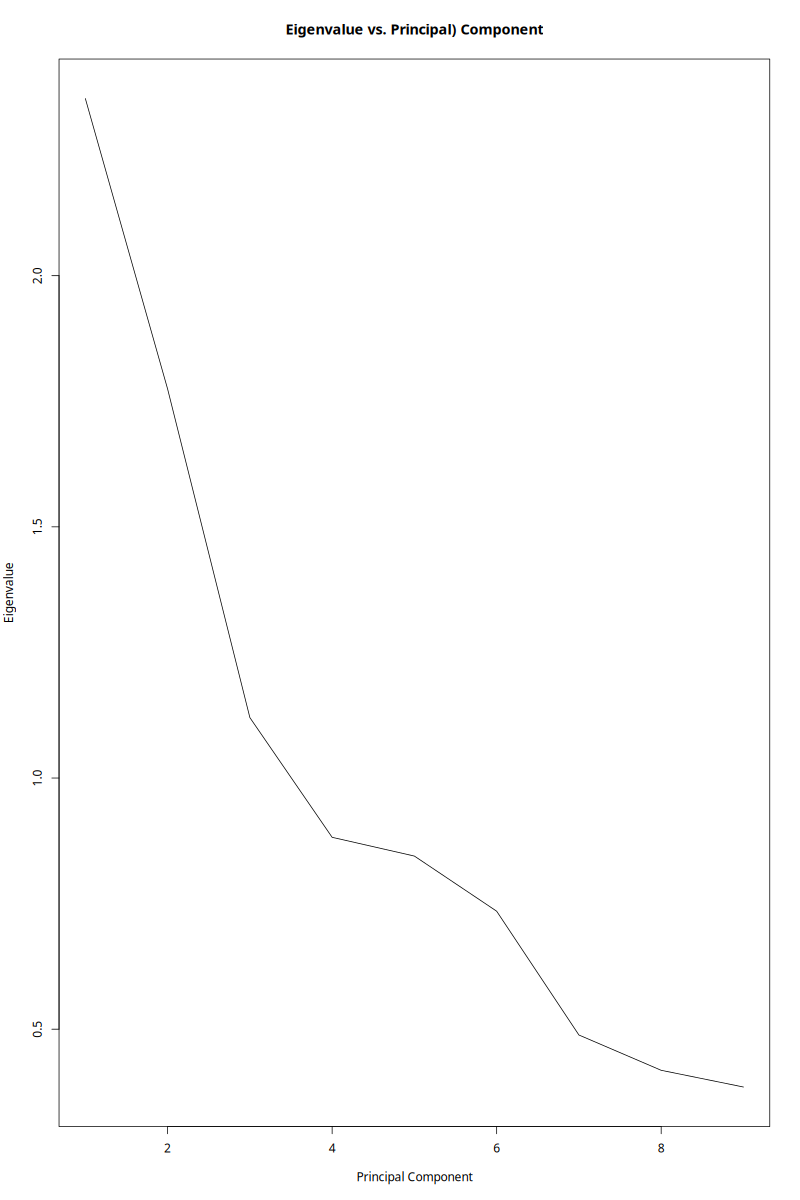
\includegraphics[width= 0.60\textwidth, height = 65mm]{eigenvalues_plot.png}\\
%     \caption{Plot of the eigenvalues}
% \end{figure}


\paragraph{QQ-plot}

From figure 2, we observe that the dataset is not normal


...... 
\subsubsection{Data Preparation} 

We write about the training and testing here?\\

.........
\section{Methodology}
\subsection{Supervised learning} 
 In this paper, we performed supervised learning methods several supervised learning methods, these methods include: Classification trees, k-nearest neighbour bagging and random forest classfiers.\cite{zhou2012ensemble}
 \subsubsection{Classification tree}

 \subsubsection{k-nearest neighbours}

 \subsubsection{bagging}

 \subsubsection{random forest classfiers}

\subsection{Binary Logistic Regression}
We performed a binary logistic regression analysis, a supervised learning method, to explore the relationship between various predictor variables and the binary response variable “Outcome,” indicating the presence or absence of diabetes. The initial model incorporated eight predictor variables: Pregnancies, Glucose, Blood Pressure, Skin Thickness, Insulin, BMI, Diabetes Pedigree Function, and Age. These variables were selected based on their potential relevance to diabetes risk, informed by existing domain knowledge.\\
\setlength{\parindent}{0pt}
The objective of the analysis was to identify the most significant predictors using the backward elimination method, a stepwise regression technique. This approach began with a model including all predictors, subsequently removing variables in sequence based on the highest p-value exceeding 0.05. This systematic elimination of statistically insignificant predictors not only enhances the model’s interpretability but also minimizes the risk of overfitting, ensuring that the final model retains only variables with significant contributions to predicting the outcome.


\section{Discussion}
\subsection{Binary Logistic Regression}
\begin{table}[H]
\centering
\begin{tabular}{llllllll}
\cline{1-5}
\multicolumn{1}{|l|}{Coefficients:}             & \multicolumn{1}{l|}{Estimate}   & \multicolumn{1}{l|}{Std. Error} & \multicolumn{1}{l|}{z value} & \multicolumn{1}{l|}{Pr(\textgreater{}|z|)} &  &  &  \\ \cline{1-5}
\multicolumn{1}{|l|}{(Intercept)}              & \multicolumn{1}{l|}{-8.4398695} & \multicolumn{1}{l|}{0.8176393}  & \multicolumn{1}{l|}{-10.322} & \multicolumn{1}{l|}{\textless 2e-16}       &  &  &  \\ \cline{1-5}
\multicolumn{1}{|l|}{Pregnancies}              & \multicolumn{1}{l|}{0.1135092}  & \multicolumn{1}{l|}{0.0375672}  & \multicolumn{1}{l|}{3.021}   & \multicolumn{1}{l|}{0.00252}               &  &  &  \\ \cline{1-5}
\multicolumn{1}{|l|}{Glucose}                  & \multicolumn{1}{l|}{0.0343876}  & \multicolumn{1}{l|}{0.0042392}  & \multicolumn{1}{l|}{8.112}   & \multicolumn{1}{l|}{4.99E-16}              &  &  &  \\ \cline{1-5}
\multicolumn{1}{|l|}{BloodPressure}            & \multicolumn{1}{l|}{-0.0134342} & \multicolumn{1}{l|}{0.0059047}  & \multicolumn{1}{l|}{-2.275}  & \multicolumn{1}{l|}{0.0229}                &  &  &  \\ \cline{1-5}
\multicolumn{1}{|l|}{SkinThickness}            & \multicolumn{1}{l|}{0.0098866}  & \multicolumn{1}{l|}{0.0083722}  & \multicolumn{1}{l|}{1.181}   & \multicolumn{1}{l|}{0.23765}               &  &  &  \\ \cline{1-5}
\multicolumn{1}{|l|}{Insulin}                  & \multicolumn{1}{l|}{-0.0015283} & \multicolumn{1}{l|}{0.0009882}  & \multicolumn{1}{l|}{-1.546}  & \multicolumn{1}{l|}{0.122}                 &  &  &  \\ \cline{1-5}
\multicolumn{1}{|l|}{BMI}                      & \multicolumn{1}{l|}{0.0776662}  & \multicolumn{1}{l|}{0.0174657}  & \multicolumn{1}{l|}{4.447}   & \multicolumn{1}{l|}{8.72E-06}              &  &  &  \\ \cline{1-5}
\multicolumn{1}{|l|}{DiabetesPedigreeFunction} & \multicolumn{1}{l|}{0.8088779}  & \multicolumn{1}{l|}{0.332009}   & \multicolumn{1}{l|}{2.436}   & \multicolumn{1}{l|}{0.01484}               &  &  &  \\ \cline{1-5}
\multicolumn{1}{|l|}{Age}                      & \multicolumn{1}{l|}{0.0297298}  & \multicolumn{1}{l|}{0.0109345}  & \multicolumn{1}{l|}{2.719}   & \multicolumn{1}{l|}{0.00655}               &  &  &  \\ \cline{1-5}
\end{tabular}
\caption{Binary Logistic Regression }
\end{table}
From Table 1, the coefficient for “SkinThickness” had the highest p-value (0.23765 > 0.05), indicating it was not significantly associated with the outcome. At this stage, the misclassification rate was 0.22396. Consequently, “SkinThickness” was removed from the model. After removing “SkinThickness,” the coefficient for “Insulin” had the highest p-value (0.24334 > 0.05), indicating it was also not significant. Then 'insulin' was excluded from the model.\\
\begin{table}[H]
\centering
\begin{tabular}{llllllll}
\cline{1-5}
\multicolumn{1}{|l|}{Coefficients:}            & \multicolumn{1}{l|}{Estimate}  & \multicolumn{1}{l|}{Std. Error} & \multicolumn{1}{l|}{z value} & \multicolumn{1}{l|}{Pr(\textgreater{}|z|)} &  &  &  \\ \cline{1-5}
\multicolumn{1}{|l|}{(Intercept)}              & \multicolumn{1}{l|}{-8.304974} & \multicolumn{1}{l|}{0.80035}    & \multicolumn{1}{l|}{-10.377} & \multicolumn{1}{l|}{\textless 2e-16}       &  &  &  \\ \cline{1-5}
\multicolumn{1}{|l|}{Pregnancies}              & \multicolumn{1}{l|}{0.115468}  & \multicolumn{1}{l|}{0.037168}   & \multicolumn{1}{l|}{3.107}   & \multicolumn{1}{l|}{0.00189}               &  &  &  \\ \cline{1-5}
\multicolumn{1}{|l|}{Glucose}                  & \multicolumn{1}{l|}{0.03207}   & \multicolumn{1}{l|}{0.003896}   & \multicolumn{1}{l|}{8.232}   & \multicolumn{1}{l|}{\textless 2e-16}       &  &  &  \\ \cline{1-5}
\multicolumn{1}{|l|}{BloodPressure}            & \multicolumn{1}{l|}{-0.012428} & \multicolumn{1}{l|}{0.005724}   & \multicolumn{1}{l|}{-2.171}  & \multicolumn{1}{l|}{0.02992}               &  &  &  \\ \cline{1-5}
\multicolumn{1}{|l|}{BMI}                      & \multicolumn{1}{l|}{0.082539}  & \multicolumn{1}{l|}{0.0163}     & \multicolumn{1}{l|}{5.064}   & \multicolumn{1}{l|}{4.11E-07}              &  &  &  \\ \cline{1-5}
\multicolumn{1}{|l|}{DiabetesPedigreeFunction} & \multicolumn{1}{l|}{0.808528}  & \multicolumn{1}{l|}{0.329062}   & \multicolumn{1}{l|}{2.457}   & \multicolumn{1}{l|}{0.01401}               &  &  &  \\ \cline{1-5}
\multicolumn{1}{|l|}{Age}                      & \multicolumn{1}{l|}{0.029419}  & \multicolumn{1}{l|}{0.010701}   & \multicolumn{1}{l|}{2.749}   & \multicolumn{1}{l|}{0.00598}               &  &  &  \\ \cline{1-5}
\end{tabular}
\caption{Binary Logistic Regression }
\end{table}
Table 2 demonstrates that all remaining variables exhibited p-values below 0.05, confirming their statistical significance. Additionally, the misclassification rate decrease to 0.21354, signaling enhanced model performance. Consequently, the variables ‘Pregnancies,’ ‘Glucose,’ ‘Blood Pressure,’ ‘BMI,’ ‘Diabetes Pedigree Function,’ and ‘Age’ were identified as having a significant influence on the “Outcome.” This suggests a strong association between these factors and the risk of diabetes in females.

\section{Conclusion}

.........

 \section{Bibliography}
 \bibliographystyle{unsrt}
 \bibliography{references}

\end{document}

